\documentclass[12pt,a4paper]{article}
\usepackage[utf8]{inputenc}
\usepackage[greek,english]{babel}
\usepackage[pdftex]{graphicx}
\usepackage[top=1in, bottom=1in, left=0.5in, right=0.5in]{geometry}
\linespread{1}
\setlength{\parskip}{4pt plus2pt minus2pt}
\widowpenalty 10000
\clubpenalty 10000
\newcommand{\eat}[1]{}
\newcommand{\HRule}{\rule{\linewidth}{0.5mm}}
\usepackage[official]{eurosym}
\usepackage{enumitem}
\setlist{nolistsep,noitemsep}
\usepackage[hidelinks]{hyperref}
\usepackage{cite}
\usepackage{lipsum}
\graphicspath{ {./images/} }
\usepackage{listings}
\usepackage{color}
\usepackage{blindtext}
\usepackage{titlesec}
\setlength{\parindent}{0pt}


\definecolor{dkgreen}{rgb}{0,0.6,0}
\definecolor{gray}{rgb}{0.5,0.5,0.5}
\definecolor{mauve}{rgb}{0.58,0,0.82}

\lstset{frame=tb,
	language=C,
	aboveskip=3mm,
	belowskip=3mm,
	showstringspaces=false,
	columns=flexible,
	basicstyle={\small\ttfamily},
	numbers=none,
	numberstyle=\tiny\color{gray},
	keywordstyle=\color{blue},
	commentstyle=\color{dkgreen},
	stringstyle=\color{mauve},
	breaklines=true,
	breakatwhitespace=true,
	tabsize=3
}

\title{ECE 450 Exam 3}
\author{Zachary DeLuca}
\date{November 4th 2023}

\begin{document}
	
	\maketitle
	\hline
	\section*{Problem Statement}
	For this exam, a filter with the following specifications and lowest order must be found. The requirements are as follows: 
	$$\omega_p \geq 400 \frac{rad}{s}\ \ \ \omega_s \leq 200 \frac{rad}{s}$$
	$$|H_p| \geq 0.9\ \ \ |H_s|\leq 0.2$$
	
	\section*{Filter Selection}
	To help choose which filter should be used, we  eliminated Chebychev I immediately, as it is non monotonic in the passband. The options left are butterworth and Chebychev II. Using the programs to find the minimum order required, the lowest orders found were: 
	$$Butterworth = 5$$
	$$Chebychev\ II= 3$$
	Given these results, the Chebychev II filter was chosen. 
	\section*{Low Pass Base}
	To start the filter design, a low pass filter with corner frequency of 1 rad/s is made. The design starts with finding $\varepsilon$, $\alpha$, and the major and minor axes of the root ellipse. 
	$$\varepsilon = \sqrt{\frac{H_s^2}{1-H_s^2}} = 0.100$$
	$$\alpha = \frac{1}{\varepsilon}+\sqrt{1+\frac{1}{\varepsilon^2}} = 19.95$$
	$$a = \frac{1}{2}\left(\alpha^{\frac{1}{n}}-\alpha^{-\frac{1}{n}}\right) = 1.17$$
	$$b = \frac{1}{2}\left(\alpha^{\frac{1}{n}}+\alpha^{-\frac{1}{n}}\right)=1.54$$
	The next step is to find the poles. There will be a single pole on the axis and a double pole at $180^{\circ}$ - $60^{\circ}$. The poles are: 
	$$s_1 = a$$
	$$s_{2,3}=acos(\theta_i) + bjsin(\theta_i)$$
	As this is the inverse Chebychev filter, the poles need to be inverted:
	$$q_{1} = \frac{1}{a}$$
	$$q_{2,3}=\frac{1}{acos(\theta_i) + bjsin(\theta_i)}$$
	
	For the numerator, the zeros are needed. As there is only one set of poles not on the axis, we need only find the one:
	
	$$\omega_k = sec\left(\frac{\pi}{6}\right)=1.15$$
	
	Once the code has run its course, we are left with a transfer function polynomial of:
	$$H(s) = K\frac{s^2+1.15^2}{s^3+0.3s^2-2.7*10^{-16}s+.4}$$
	K is found when s = 0:
	$$K = \frac{0.4}{0.15^2}=0.35$$
	When we graph this function, we get: 
	\begin{center}
		\textit{Figure 1: Low Pass Base Centered at 1 rad/sec}
		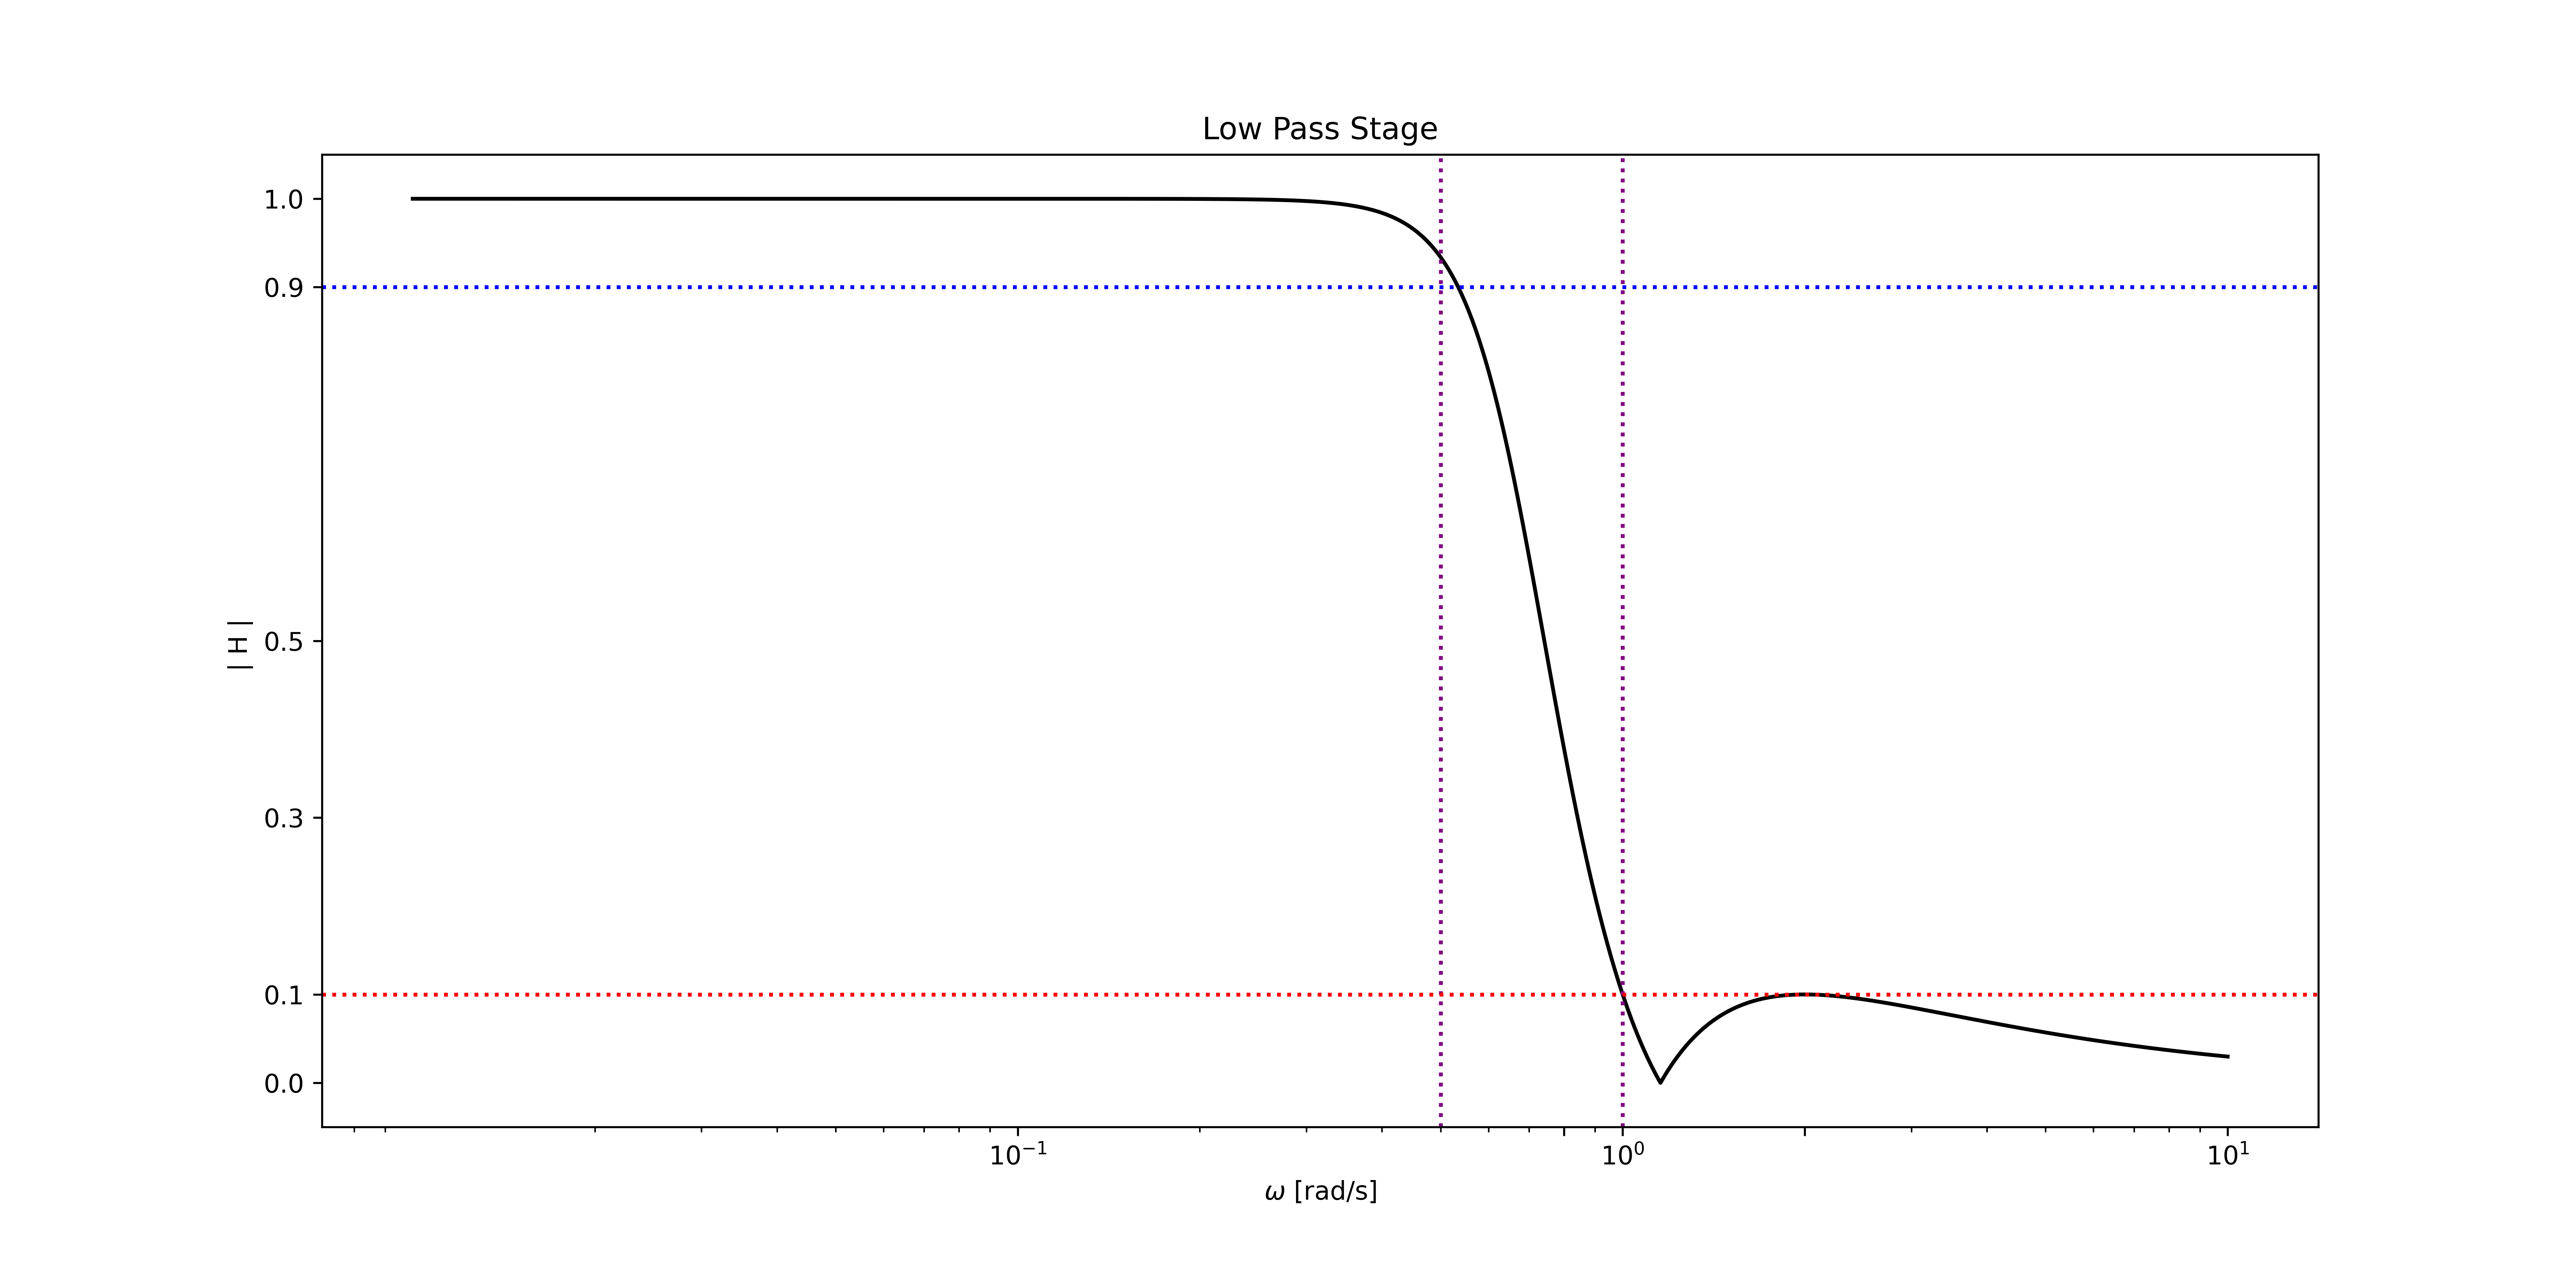
\includegraphics[width = 7in]{Figure_1.png}
	\end{center}
	\section*{High Pass Conversion}
	To convert the graph to a high pass filter, we replace each $s$ with $\frac{1}{s}$ and that yields: 
	$$H(0)=\left(\frac{\left(\frac{1}{s}\right)^2+1.15^2}{\left(\frac{1}{s}\right)^3 + 0.3\left(\frac{1}{s}\right)^2-2.7*10^{-16}\left(\frac{1}{s}\right)+0.4}\right)=K\frac{s+1.15^2s^3}{0.4s^3-2.7*10^{-16}s^2+0.3s+1}$$
	Normalizing that polynomial yields assuming K = 1 to facilitate the passband going to 1: 
	$$\frac{s^3+0.75s}{s^3-6.9*10^{-16}s^2+0.75s+2.48}$$
	If we graph this we can see that it is a flip of the low pass filter around the $\omega_s$ value at 1 rad/sec:
		\begin{center}
		\textit{Figure 2: High Pass Filter Centered at 1 rad/sec }
		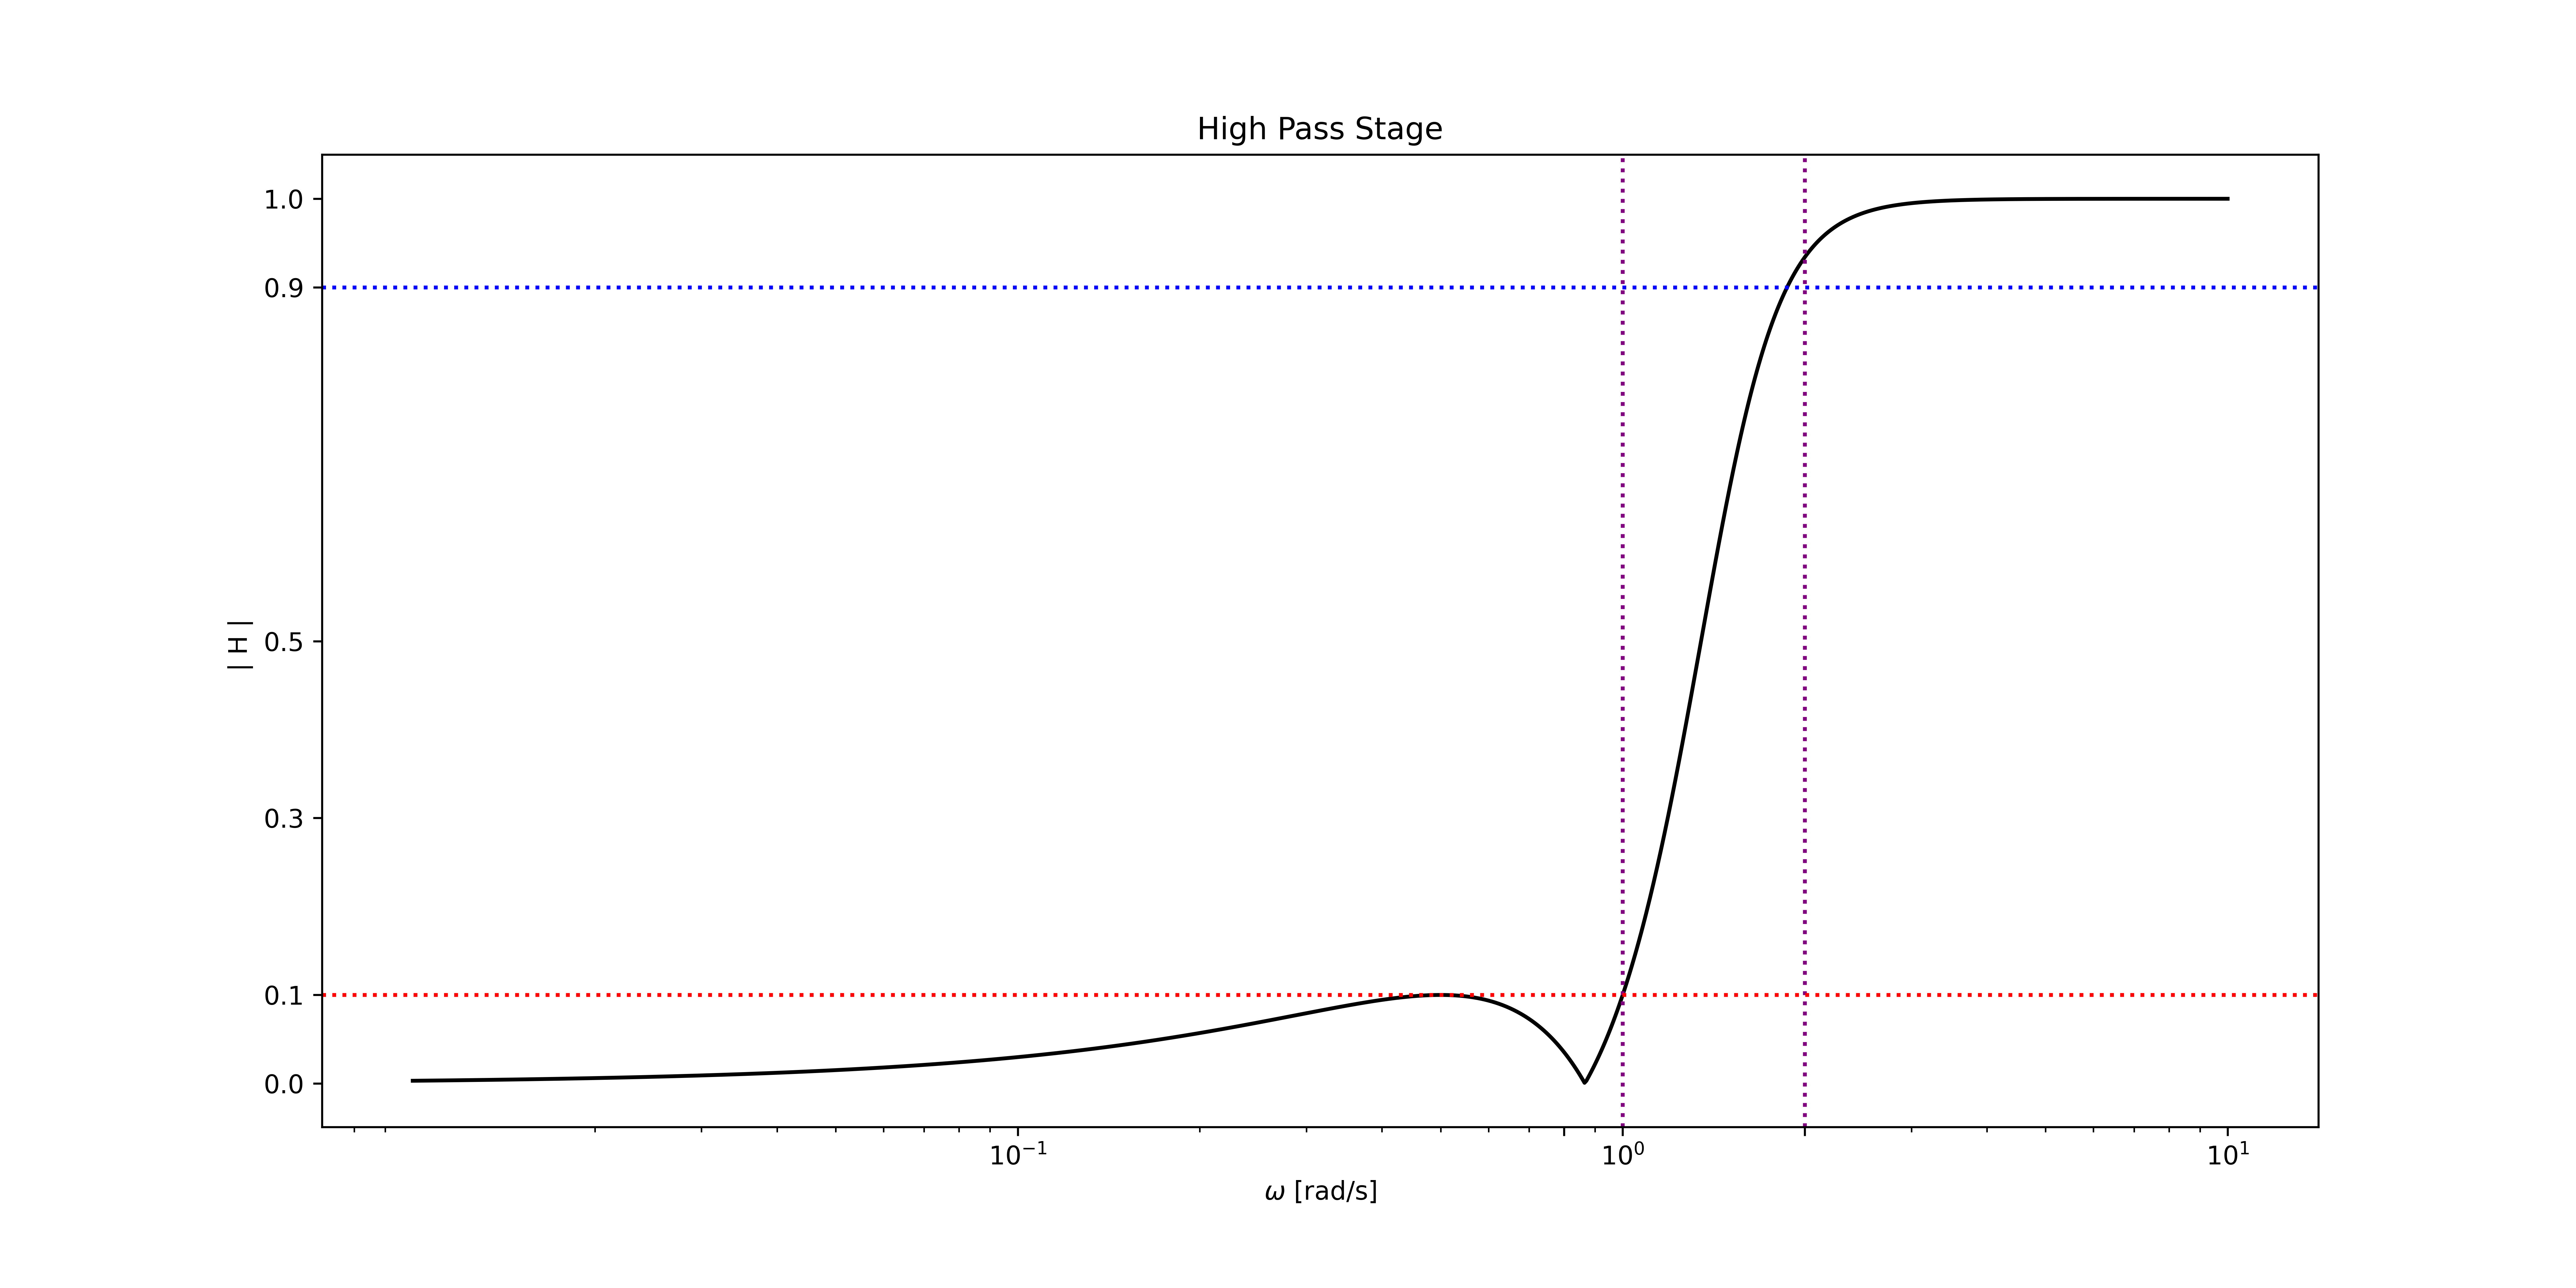
\includegraphics[width = 7in]{Figure_2.png}
	\end{center}
	\section*{Frequency Scale}
	Now that the high pass filter has been found, simply scaling the filter by 200 rad/s will shift the corner frequency to our desired criterion: 
	$$H(\frac{s}{\omega})=\frac{s^3+30000s}{s^3-1.38*10^{-13}s^2+30000s+20*10^{6}}$$
	
	Graphing this will show how the function retains its shape and has moved to meet the requirements of the problem statement: 
	If we graph this we can see that it is a flip of the low pass filter around the $\omega_s$ value at 1 rad/sec:
	\begin{center}
		\textit{Figure 3: High Pass Filter Centered at 200 rad/sec }
		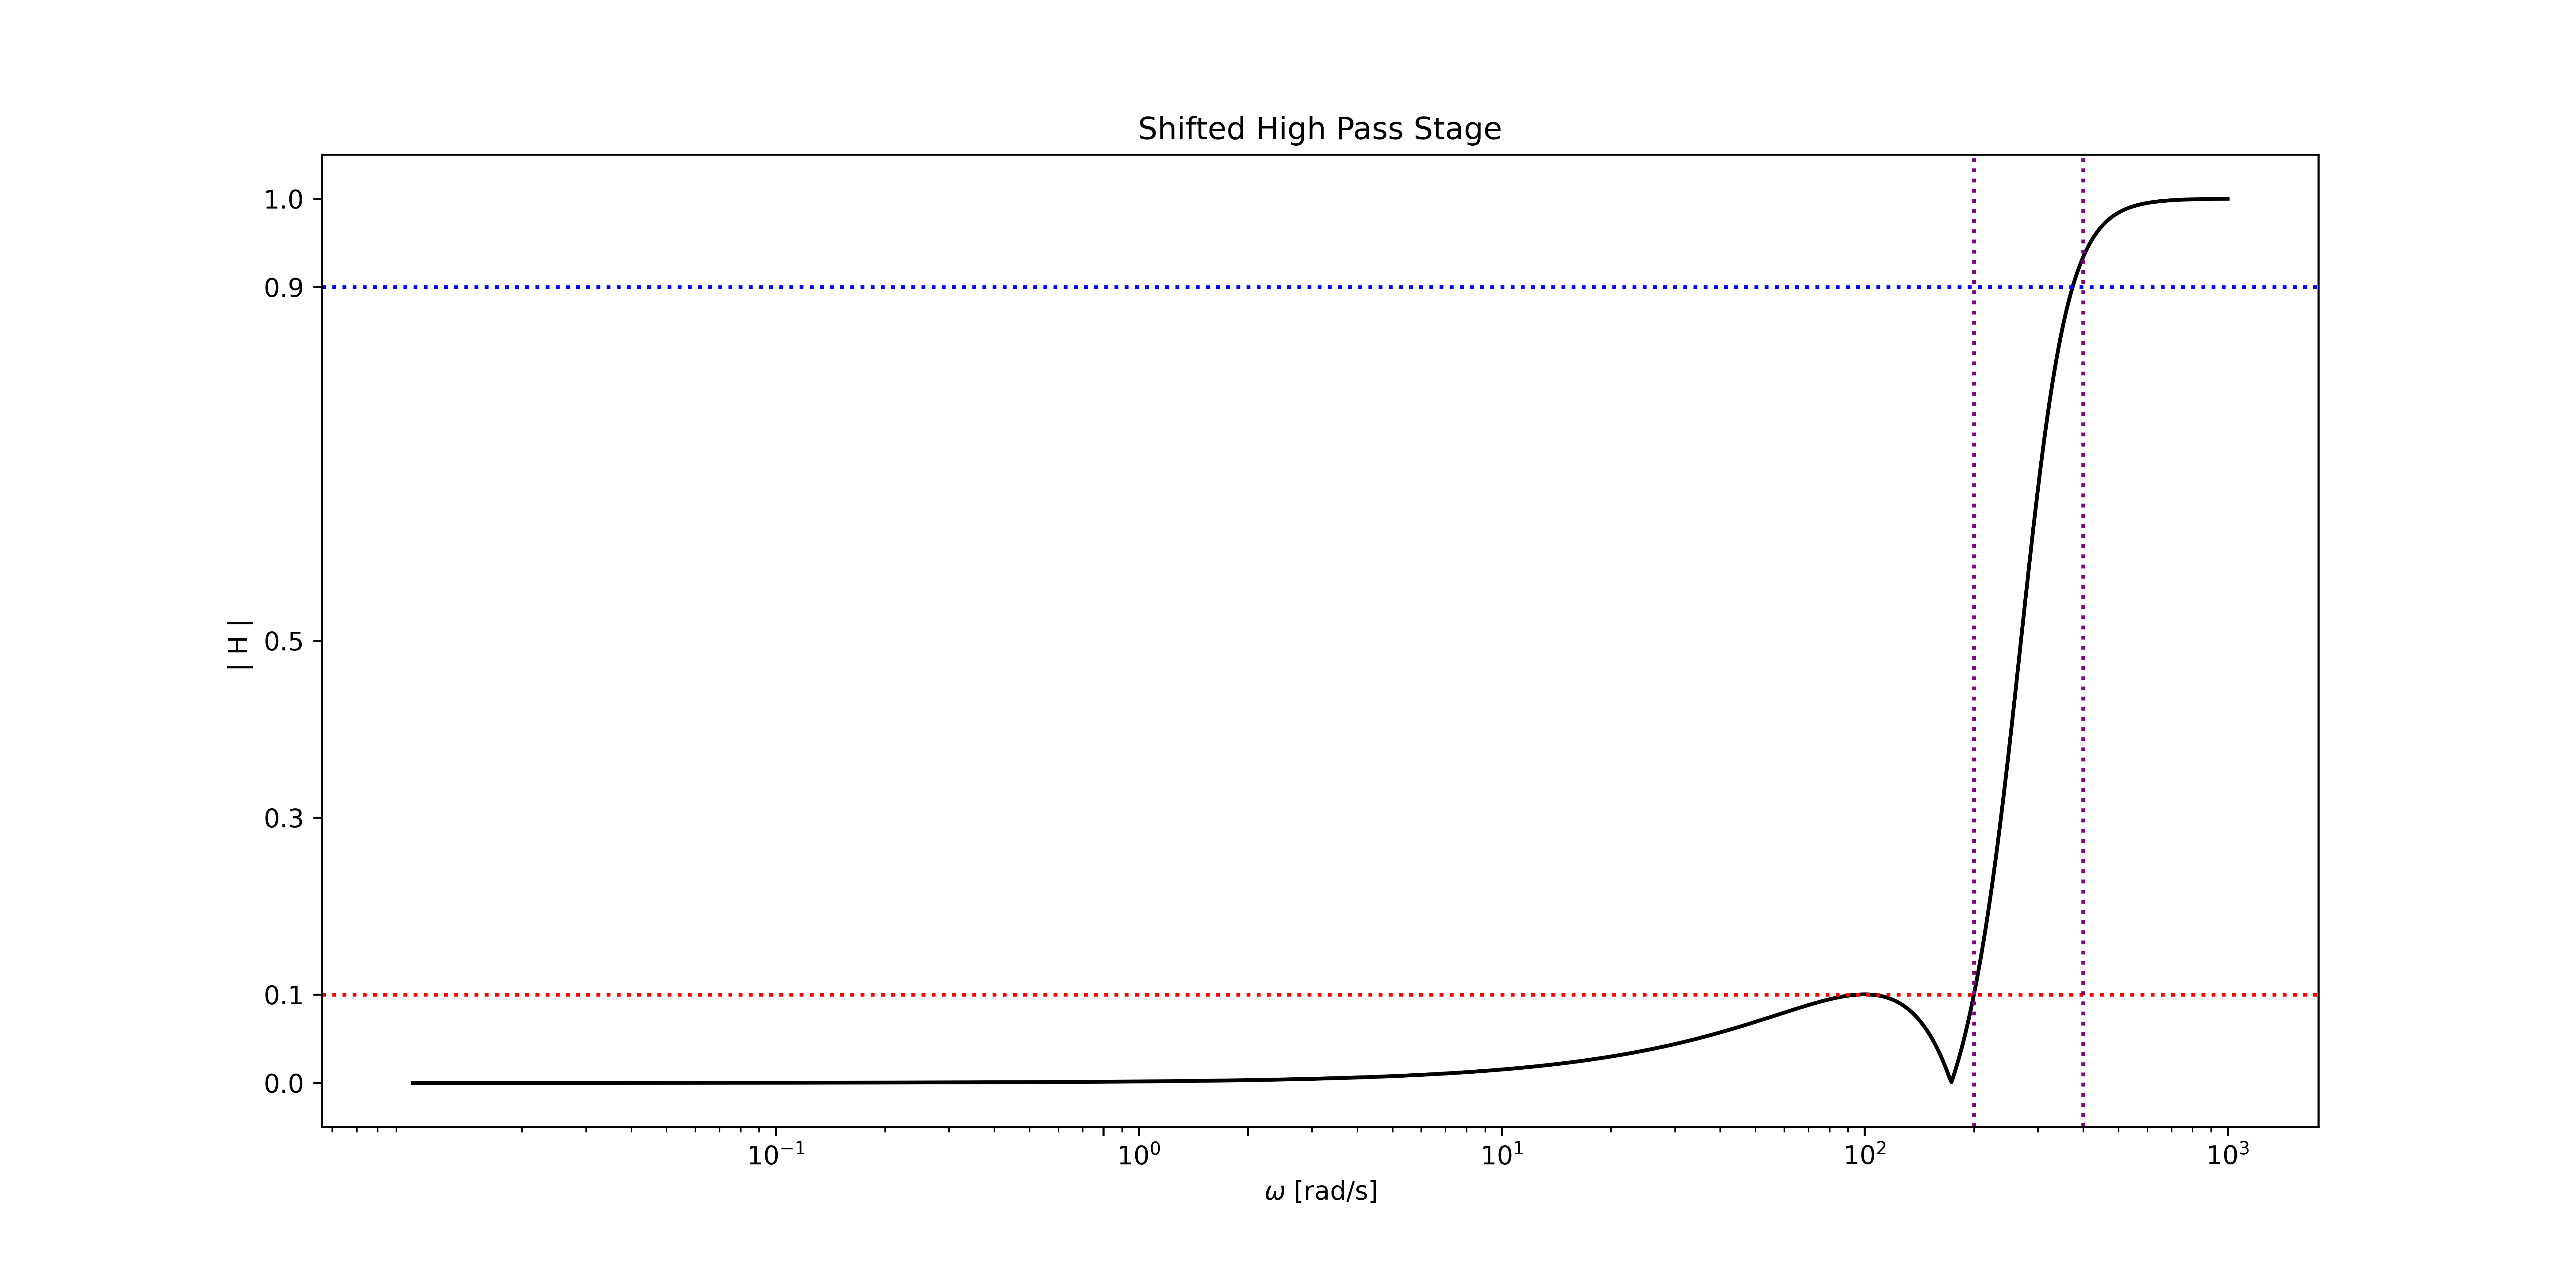
\includegraphics[width = 7in]{Figure_3.png} \vspace*{12pt}
		
		\textit{Figure 4: High Pass Filter Zoomed into Area of Interest}
		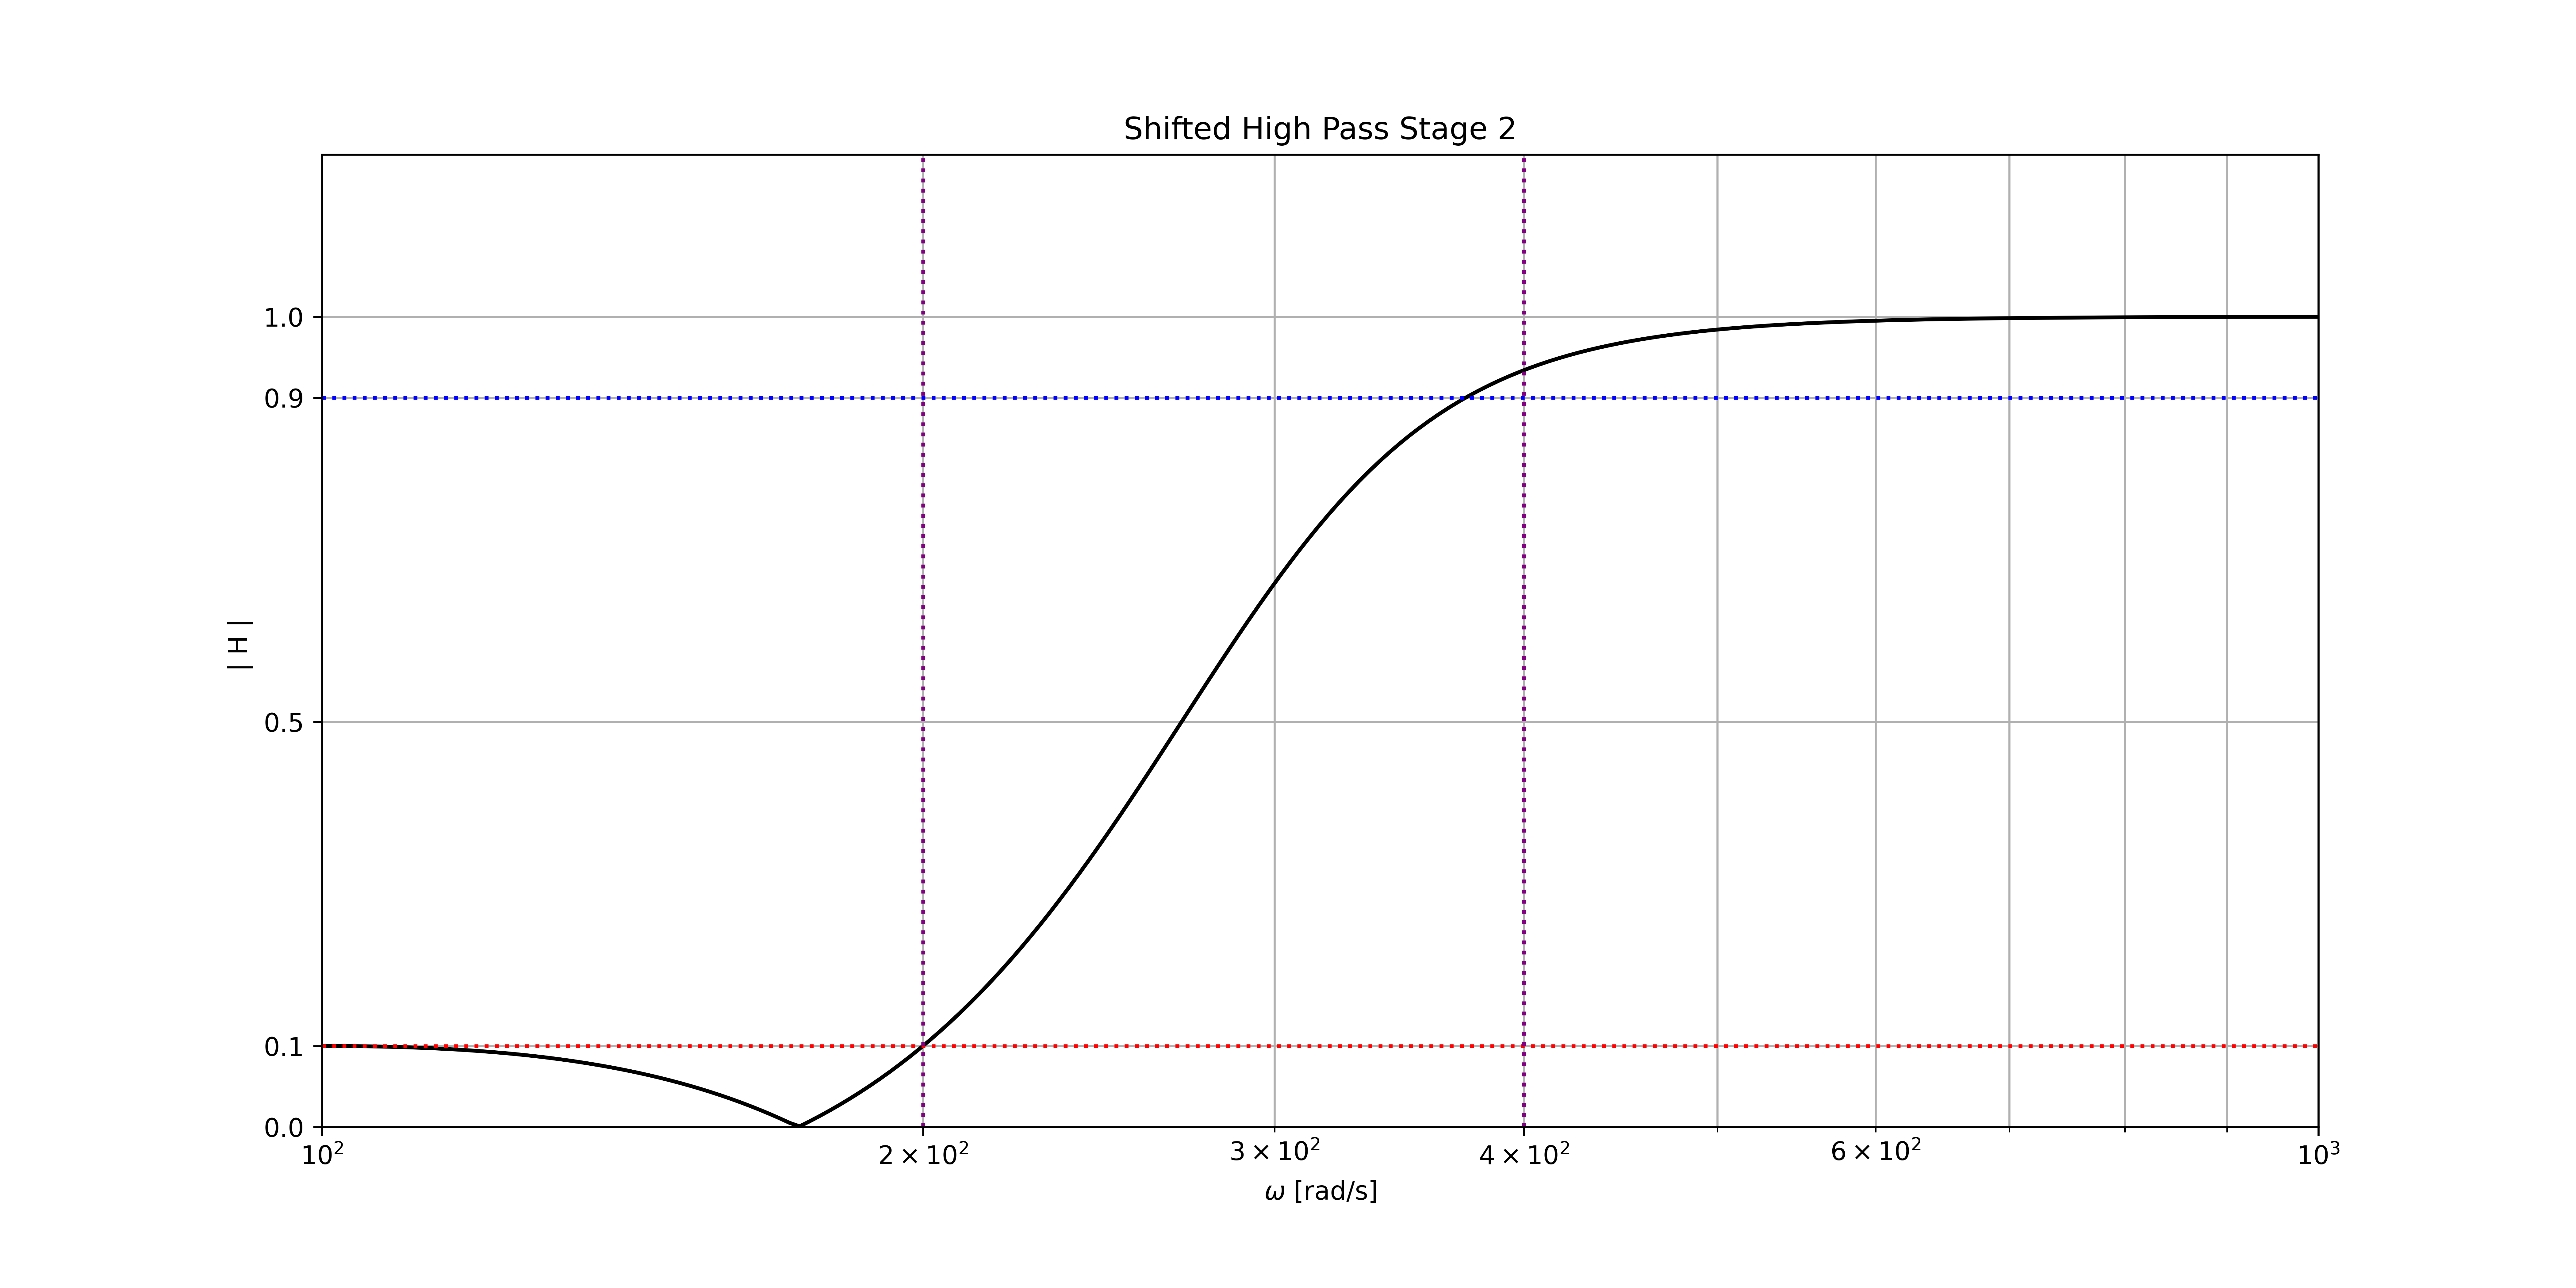
\includegraphics[width = 7in]{Figure_4.png} 
	\end{center}
	To verify the filter, time domain graphs were creating showing what happens at 200 rad/sec and 400 rad/sec (The blue lines represent the outputs):
	
		\begin{center}
		\textit{Figure 5: Filter Output at 200 rad/sec }
		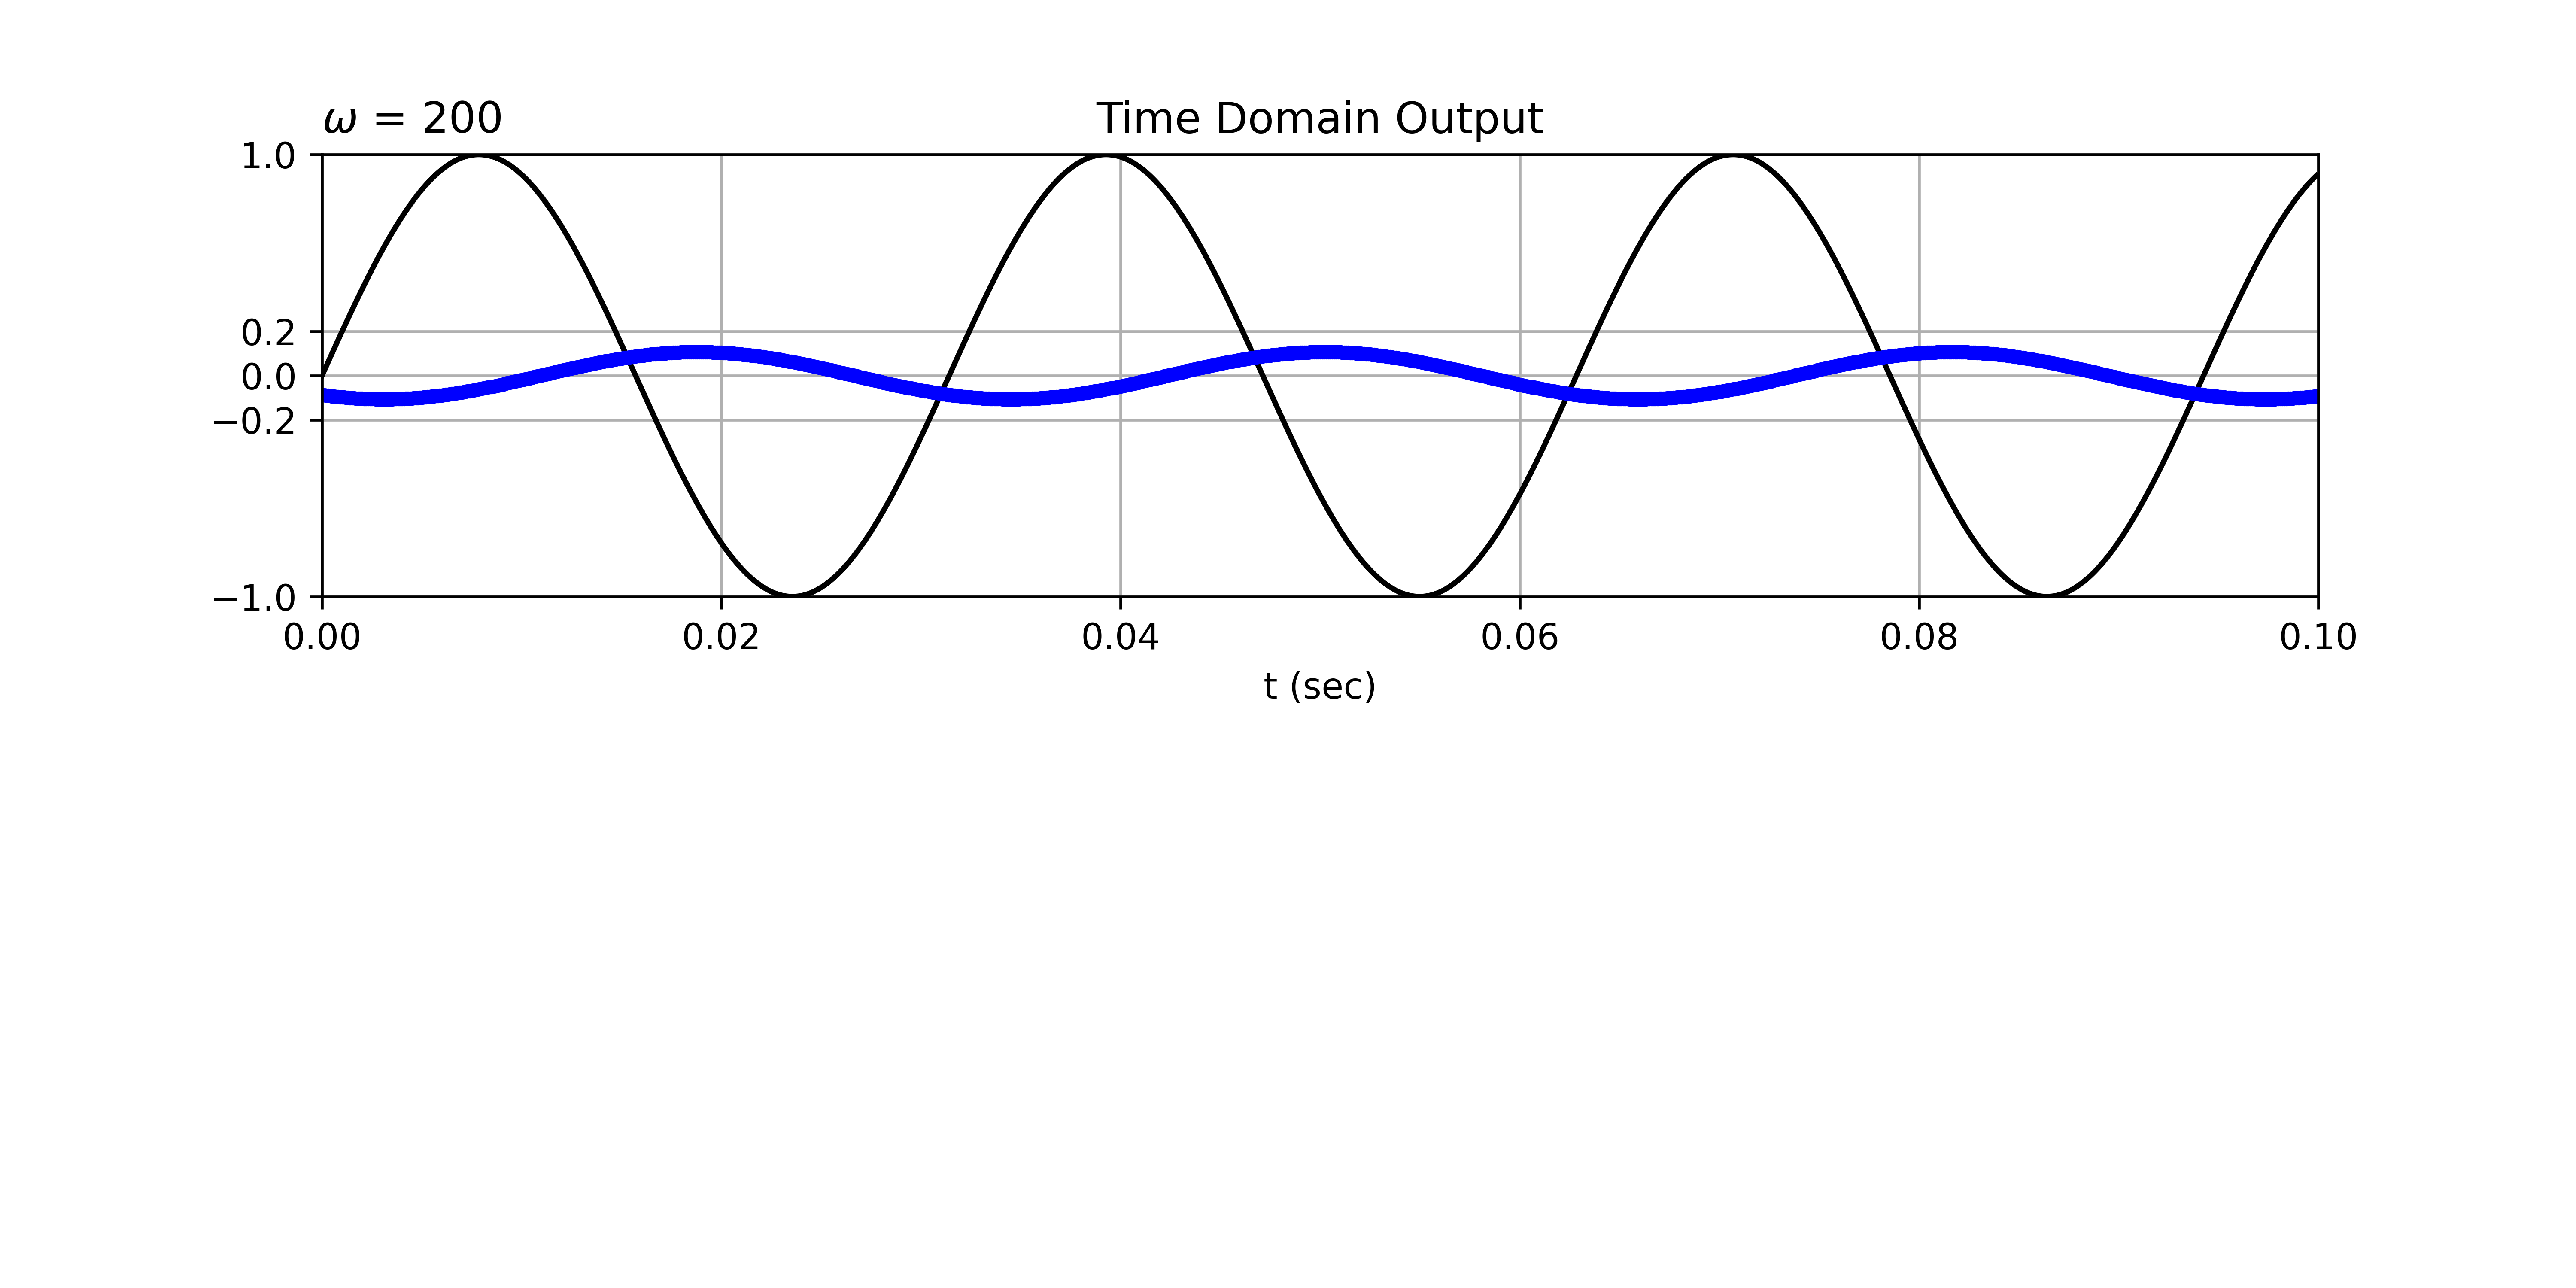
\includegraphics[width = 7in]{Figure_5.png} \vspace*{12pt}
		
		\textit{Figure 6: Filter output at 400 rad/sec}
		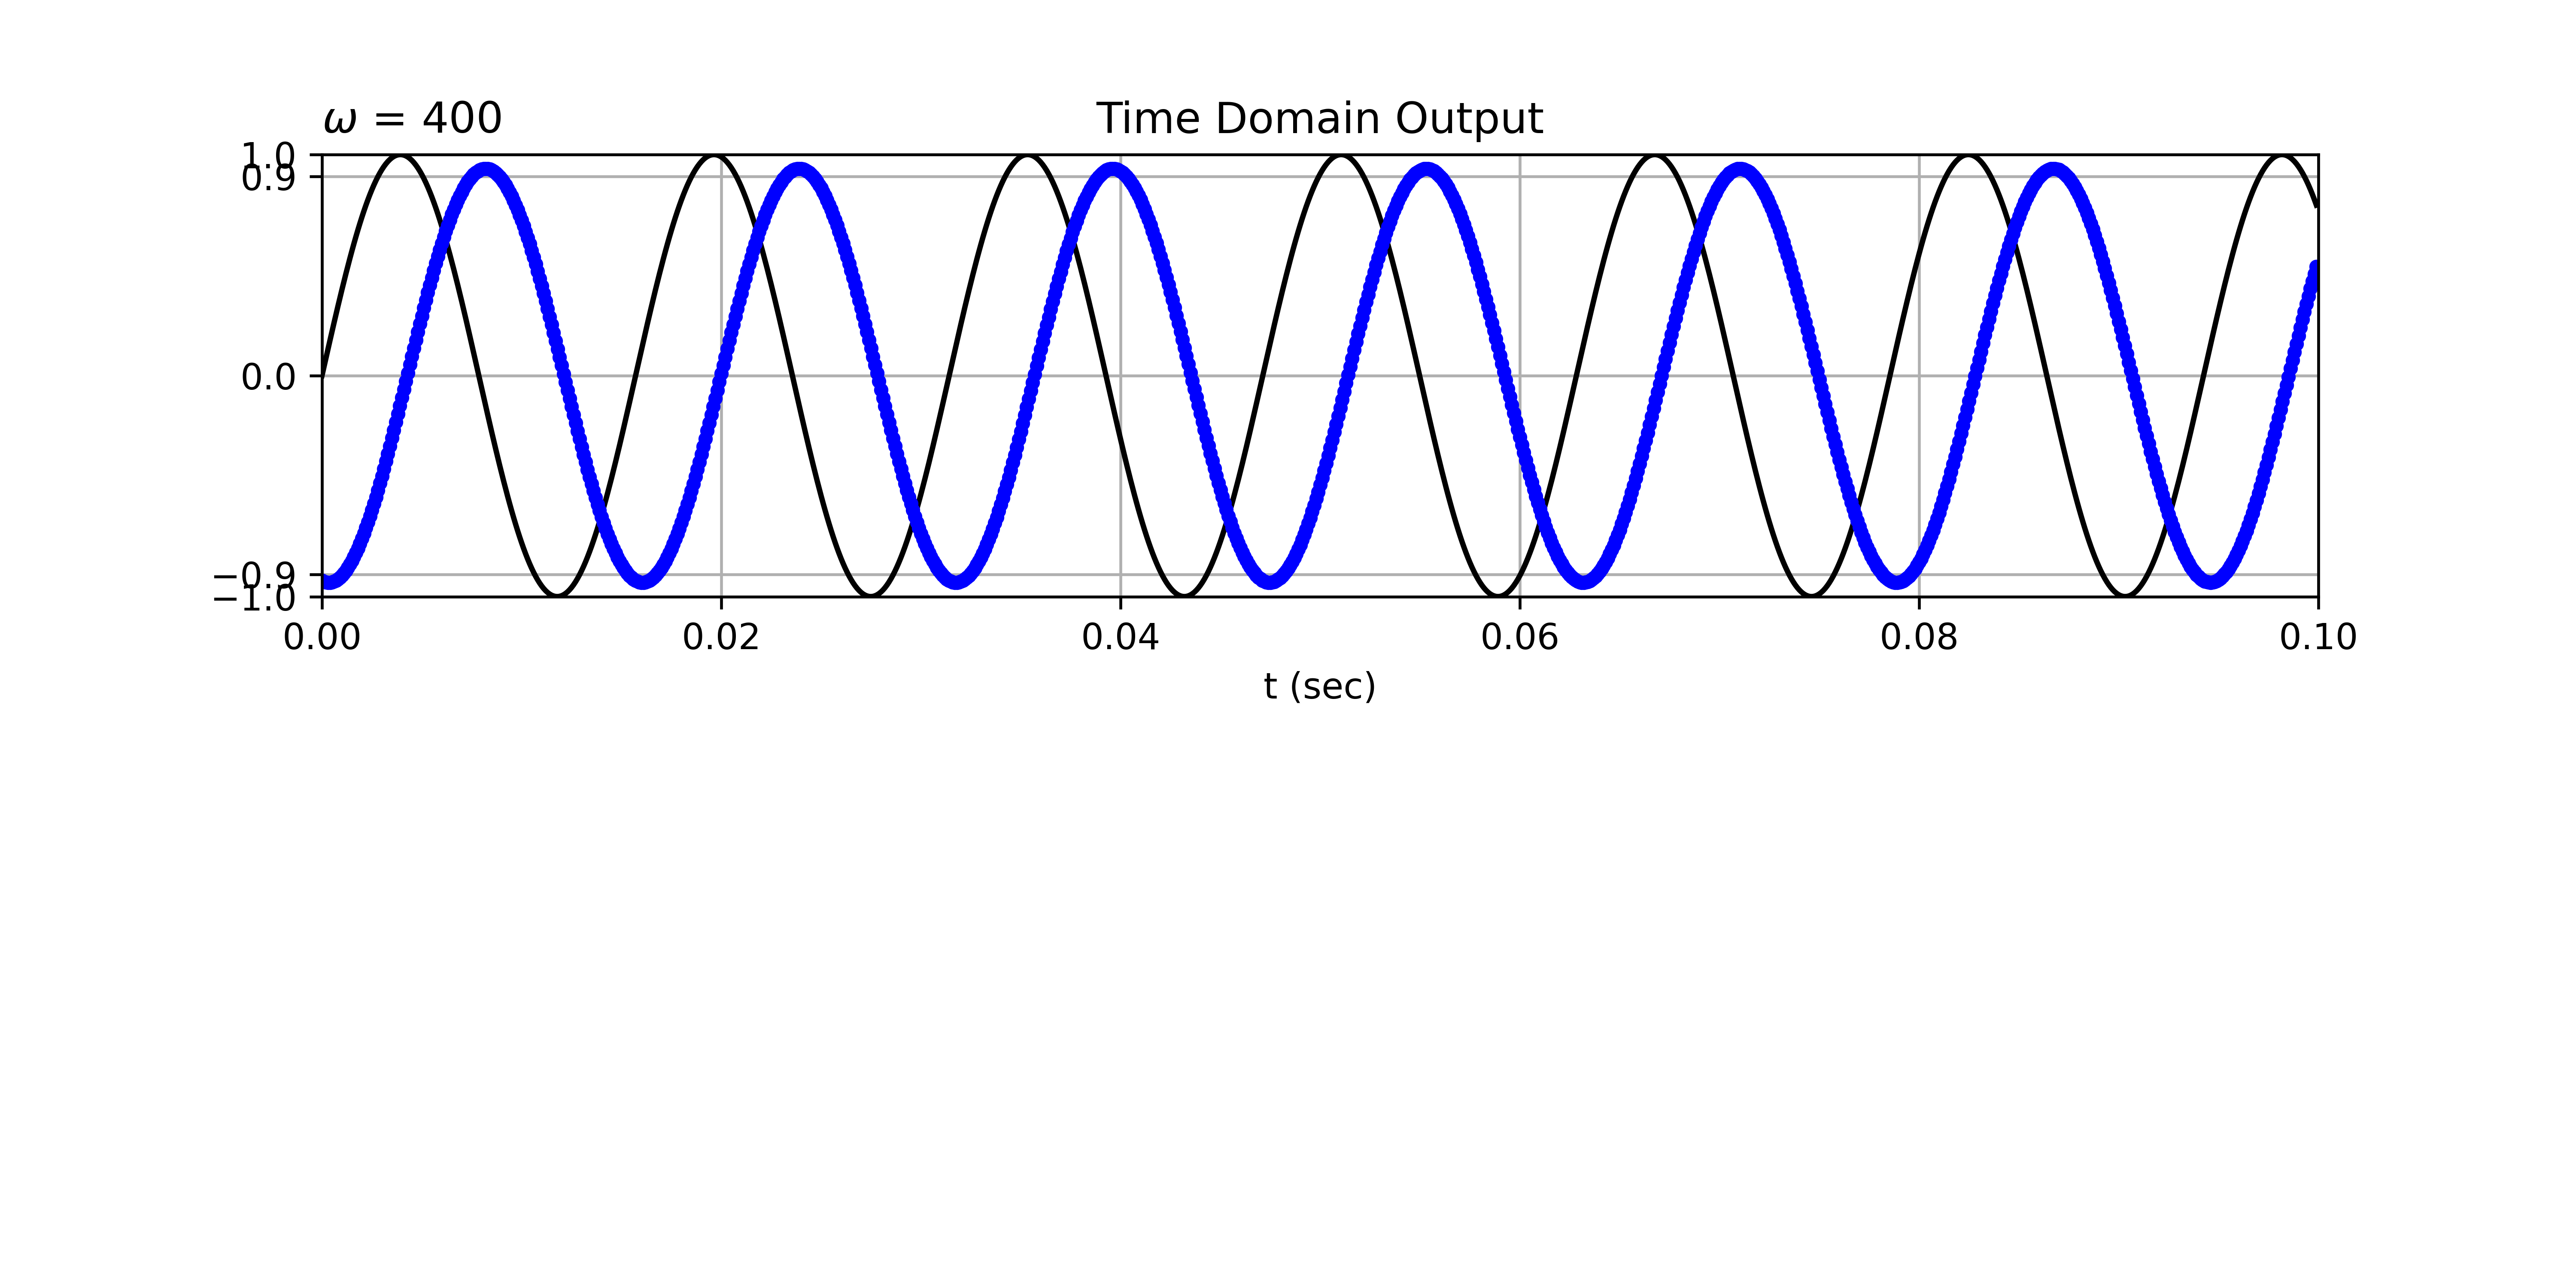
\includegraphics[width = 7in]{Figure_6.png} 
	\end{center}
	\section*{Conclusion}
	The filter made was much more complicated to create and simulate than a butterworth version, but the chosen filter was able to do the same with a two degree lower filter. The graphs of the magnitude give important verification that the filters were designed correctly at each stage. 
	
\end{document}